\section{Implementation}
\label{sec:implementation}

\iffalse TODO:
  A: Conceptually: - implementation follows the inductive/recursive structure of the previous definitions
e.g. definition of the rose tree is naturally represented as Haskell datatype definition

B Module-by-module road map
  - Treatment of Haskell package system

C - External software
\fi

We provide an implementation of our recurrent clustering algorithm in a tool called \textsc{ML4HS}, which consists of a loose collection of components shown in Figure \ref{fig:ml4hs}. This arrangement makes it easy to swap out parts for experimentation. In the following, we describe the custom components in the order they appear in the diagram.

\begin{figure}
  \centering
  \tikzstyle{block} = [rectangle, draw, rounded corners]
  \tikzstyle{container} = [rectangle, draw, rounded corners]
  \tikzstyle{line} = [draw, -latex']
  \colorlet{shade}{rgb:black,1;white,4}

  \begin{tikzpicture}[node distance=2cm]
    \node [block] (hackage) {Hackage};

    \node [block, below of=hackage] (cabal) {
      \begin{tikzpicture}[node distance = 2cm]
        \node (caballabel) {Cabal};
        \node [block, anchor=north west] at (caballabel.south) (ghc) {
          \begin{tikzpicture}[node distance = 2cm]
            \node (ghclabel) {GHC};
            \node [block, anchor=north west, fill=shade] at (ghclabel.south) (plugin) {AST Plugin};
          \end{tikzpicture}
        };
      \end{tikzpicture}
    };

    \node [block, below of=cabal, fill=shade]  (sorting) {Sorting};

    \node [block, below of=sorting, fill=shade] (clustering) {
      \begin{tikzpicture}[node distance = 2cm, auto]
        \node (clusterlabel) {Recurrent Clustering};
        \node [block, anchor=north west, fill=shade] at (clusterlabel.south west) (fe) {Feature Extraction};
        \node [block, anchor=west, fill=white] at ([xshift=2em]fe.east) (weka) {Weka};

        \path [line] (fe)   -- (weka);
        \path [line] (weka) -- (fe);
      \end{tikzpicture}
    };

    \node [block, below of=clustering, fill=shade] (mlspec) {
      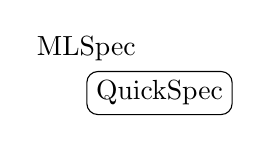
\begin{tikzpicture}[node distance = 2cm, auto]
        \node (mlspeclabel) {MLSpec};
        \node [block, anchor=north west, fill=white] at (mlspeclabel.south) (qs) {QuickSpec};
      \end{tikzpicture}
    };

    \node [block, below of=mlspec] (user) {User};

    \path [line] (hackage)    -- (cabal);
    \path [line] (cabal)      -- (sorting);
    \path [line] (sorting)    -- (clustering);
    \path [line] (clustering) -- (mlspec);
    \path [line] (mlspec)     -- (user);
  \end{tikzpicture}
  \caption{Components of the ML4HS theory exploration system. Custom components are shaded, arrows indicate data flow.}
  \label{fig:ml4hs}
\end{figure}

\subsection{\textsc{ASTPlugin}}
\label{sec:astplugin}

The GHC compiler provides mechanisms for parsing Haskell source code and converting it to Core. It also includes a \emph{renaming} transformation which makes all names unique (either by prefixing them with the name of the module which defines them, or by suffixing the name with a number. This allows us to spot repeated use of a term, across multiple modules and packages, with a simple syntactic equality check.

Since we are interested in comparing definitions based on the terms they reference, building our framework on top of GHC seems like a promising approach. Indeed, \hspec{} already invokes GHC's API to obtain the definitions of Haskell functions, in order to transform them into a form suitable for ATP systems. However, our initial experiments showed that this technique is too fragile for use on many real Haskell projects.

This is due to many projects having a complex module structure, requiring particular GHC flags to be given, or using pre-processors such as \texttt{cpp} and Template Haskell to generate parts of their code. All of this complexity means that invoking GHC ``manually'' via its API is unlikely to obtain the definitions we require.

Thankfully there is one implementation detail which most Haskell packages agree on: the Cabal build system. All of the above complexities will be specified in a package's ``Cabal file'', such that the \texttt{cabal configure} and \texttt{cabal build} commands are very likely to work for most packages, without any extra effort. This shifted our focus to augmenting GHC and Cabal, such that definitions can be collected during the normal Haskell build process.

GHC provides a plugin mechanism for manipulating Core during a build, intended for optimisation passes, which we use to inspect definitions as they are being compiled. We provide a plugin called \textsc{AstPlugin} which emits a serialised version of each Core definition to the console (to satisfy the type system, it also implements a dummy ``optimisation'' which returns the Core unchanged).

Compared to Haskell, Core is a much simpler language and its representation is relatively stable compared to many existing representations of Haskell (which often change to support various language extensions). Three areas which make Core difficult to handle are:

\begin{description}
  \item{Type variables}: Parametric polymorphism (described in more detail in \S \ref{sec:haskelldesc}) can be thought of as values being parameterised by type-level objects. In System F, this is represented explicitly by a special abstraction form $\Lambda$, distinct from the $\lambda$ used for values. Core only has one abstraction form, \CLam, for both types and values. This alters function properties like arity.

  \item{Unified namespace}: Haskell has distinct namespaces for values, types, data constructors, etc. Since Core does not make these distinctions, names may become ambiguous. For example, a type parameter \hs{t} may be confused with a function argument \hs{t}. To prevent this, overlapping namespaces are distinguished by prefices which are distinct from the available names; for example a type class constraint \hs{Ord t} may give rise to a binder $\CLam\ \hs{"\$dOrd"}$ in Core. This causes difficulties when looking up names, as these prefixed forms do not easily map back to the Haskell source.

  \item{Violating encapsulation}: Although Haskell allows names to be \emph{private} to a module, when compiling Core we have full access to private definitions, as well as references to private names from within other definitions. Hence the definitions we receive from \textsc{AstPlugin} will include private values which we cannot import into a theory exploration tool.
\end{description}

In practice, we work around these issues with a post-processing stage: for each named definition appearing in the output of \textsc{AstPlugin}, we attempt to reference that name within the GHCi interpreter. Names with the above problems will cause an error, and are discarded.

The result of building a Haskell package with \textsc{AstPlugin} is a database of Haskell definitions, similar in some respects to \textsc{Hoogle}. Definitions are indexed by a combination of their package name, module name and binding name. The definitions themselves are s-expressions representing the Core AST, with non-local references replaced by a combination of package name, module name and binding name, which allows dependencies to be discovered. Each definition also has an associated arity and type, obtained during the post-processing step mentioned above.

\subsection{Toplogical Sorting}

As described in \S \ref{} We have a tool which annotates each definition with its dependencies, i.e. those (package, module, name) combinations which it references. Definitions are then topologically sorted into dependency order, as this is required for our recurrent clustering technique.

\subsection{Recurrent Clustering}

\iffalse TODO: maybe focus on the ``interesting cases'', and defer the nitty-gritty of extending the environment, etc. to the implementation section? \fi

Our implementation is a rather direct translation of the algorithm described in \S \ref{sec:contributions} into Haskell. At the top level, we send named expressions to \hs{recurrentCluster}, topologically sorted: if an element contains multiple \hs{(Global, Expr)} pairs, they are mutually-recursive:

\begin{haskell}
recurrentCluster :: [[(Global, Expr)]] -> [[Global]]
recurrentCluster = go ([],[])
  where go (fs, db) []       = db
        go (fs, db) (es:ess) = let fs' = fs ++ map (extract db) es
                                   db' = kMeans fs'
                                in go (fs', db') ess
        extract db (i, e) = (i, rt db e)
\end{haskell}

The overall result of the \hs{recurrentCluster} function is a list of clusters, containing the IDs of their elements. These are obtained by interleaving clustering (the \hs{kMeans} function) and feature extraction (the \hs{rt} function).

The feature extraction itself contains two parts: first, syntax trees matching the grammar in Figure \ref{fig:coresyntax} are converted into \hs{RoseTree}s with features (\hs{Float}s) on their \hs{Node}s:

\begin{haskell}
data RoseTree = Node Feature [RoseTree]

eRT :: [Local] -> [[Global]] -> Expr -> RoseTree
eRT env db e = case e of
  ...
\end{haskell}

The easiest branches to handle are literals and types, which we represent using particular feature values (\hs{sLITNUM}, \hs{sLITSTR} and \hs{sTYPE}):

\begin{haskell}
  Lit (LitNum _) -> Node sLITNUM []
  Lit (LitStr _) -> Node sLITSTR []
  Type           -> Node sTYPE   []
\end{haskell}

Function application simply recurses into both sub-expressions:

\begin{haskell}
  App e1 e2 -> Node sAPP [eRT env db e1,
                          eRT env db e2]
\end{haskell}

To look up variables locally and globally, we use the \hs{lookupL} and \hs{lookupG} functions, respectively. These return the index containing their argument, if found. In the case of \hs{lookupL}, this acts as a de Bruijn index to give alpha-equivalent terms equal feature vectors. For \hs{lookupG}, this is the ID of the cluster it appears in; this ensures that references to similar expressions result in similar features:

\begin{haskell}
  Var (Global i) -> Node (lookupG db  i) []
  Var (Local  i) -> Node (lookupL env i) []
\end{haskell}

Finally, when we traverse binders we must extend the environment \hs{env}:

\begin{haskell}
  Lam  i  e     -> Node sLAM [eRT (i:env) db e]
  Let  bs e     -> Node sLET (map (bRT (ids bs:env) db) bs ++
                                   eRT (ids bs:env) db  e
  Case e i alts -> Node sCASE (eRT    env  db  e :
                          map (aRT (i:env) db) alts)
\end{haskell}

Patterns and bindings are handled in a similar way:

\begin{haskell}
aRT :: [Local] -> [[Global]] -> Alt -> RoseTree
aRT env db alt = case alt of
  (DataAlt _, vs, e) -> eRT (vs ++ env) db e
  (LitAlt  _, _,  e) -> eRT env db e
  (Default,   _,  e) -> eRT env db e

bRT :: [Local] -> [[Global]] -> Bind -> RoseTree
bRT env db b = case b of
  NonRec i e -> eRT env db e
  Rec es     -> Node sREC (map (eRT env db . snd) es)
\end{haskell}

The result of \hs{eRT} is a \hs{RoseTree} whose branching structure mimics that of our original expression. We next need to convert this to a \emph{matrix} of features, which we do by converting each level of the \hs{RoseTree} into a row of the matrix (using \hs{pad} to ensure a consistent size). Finally we turn the matrix into a \emph{feature vector} by concatenating the rows:

\begin{haskell}
level :: Int -> RoseTree -> [Feature]
level 0 (Node x xs) = [x]
level n (Node x xs) = concatMap (level (n-1)) xs

rt :: [[Global]] -> Expr -> [Feature]
rt db e = concat (pad cols (map (`level` eRT [] db e) [0..rows]))
\end{haskell}

Notice that this algorithm contains several parameters, including \hs{rows} and \hs{cols} which determine how to truncate the matrices (defaults are 30). The \hs{kMeans} function also contains a parameter for the cluster number; we set this as $\sqrt{n}$ where $n$ is the number of feature vectors being clustered.

\iffalse TODO: How does this section differ from Algorithm in Contributions? \fi
\iffalse TODO: Make this a concrete presentation of the abstract ideas from the Algorithm section, e.g. this is how we get the dependencies (AST plugin, etc.); this is a case-by-case of how we perform feature extraction; this is how we perform k-means (Weka), etc. \fi

Most of the work carried out so far has been either preliminary investigations, to determine if a particular approach is worth pursuing; or at an infrastructure level to support experimentation.

\subsection{\textsc{ML4HS}}
\label{sec:ml4hs}

\textsc{ML4HS} is our top-level theory exploration framework, combining \textsc{AstPlugin} and \textsc{MLSpec}, described below, with an implementation of our recurrent clustering algorithm and the \textsc{Weka} machine learning library.

\subsection{\textsc{MLSpec}}
\label{sec:mlspec}

When investigating heuristic methods like those of machine learning, it is important to use as much realistic data as possible to predict the system's performance on real tasks. One bottleneck for theory exploration is the lack of theories which are available to explore: we must manually select a set of terms to explore, and sometimes specify variables too.

Our \textsc{MLSpec} tool can automatically build theories suitable for exploration by \qspec{}, based on the databases constructed by \textsc{AstPlugin} described above. Features of \textsc{MLSpec} include:

\begin{itemize}
  \item{Monomorphising}: Given values of polymorphic type, e.g. \hs{safeHead :: forall t. [t] -> Maybe t} and \hs{[] :: forall t. [t]}, a testing-based system like \qspec{} is unable to evaluate expressions such as \hs{safeHead [] :: forall t. Maybe t} without instantiating the variable \hs{t} to a specific type. Such an instantiation is called \emph{monomorphising}, and in the case of \textsc{MLSpec} we build on previous work in \qcheck{} by attempting to instantiate all type variables to \hs{Integer}. We discard those cases where this is invalid, such as variable \emph{type constructors} (e.g. \hs{forall c. c Bool -> c Bool}) or incompatible class constraints (e.g. \hs{forall t. IsString t => t}).

  \item{Qualification}: All names are \emph{qualified} (prefixed by their module's name), to avoid most ambiguity. There is still the possibility that multiple packages will declare modules of the same name, in which case the exploration process will abort.

  \item{Variable definition}: Once a \qspec{} theory has been defined containing all of the given terms, we inspect the types it references and append three variables for each to the theory (enough to discover laws such as associativity, but not too many to overflow the limit of \qspec{}'s exhaustive search).

  \item{Sandboxing}: \textsc{MLSpec} is built on top of \texttt{nix-eval}, which allows the theory being explored to reference packages which aren't yet installed on the system.

\end{itemize}

\subsection{\texttt{nix-eval}}
\label{sec:nixeval}

To facilitate theorem proving and machine learning, our theory exploration experiments require access to the \emph{definitions} of the terms under investigation. This is difficult, as many terms are functions, which Haskell does not let us inspect. This limitation can be worked around by programming at a meta-level: manipulating \emph{representations} of Haskell expressions, rather than the expressions themselves. To retain our ability to \emph{evaluate} expressions, we then need a mechanism to transform these representations into the expressions they represent; this usually takes the form of an \texttt{eval} function.

\texttt{eval} is a common feature in languages such as Python and Javascript, where extra source files can be imported dynamically. In that case \texttt{eval} can be implemented easily by representing expressions as strings, then treating those strings as if they were the content of a file being imported.

On the other hand, Haskell does not natively support dynamic importing of extra source files, making implementation of \texttt{eval} trickier. Comprehensive implementations do exist, such as \texttt{hint}, which are effectively wrappers around GHC, but all are limited to using the Haskell modules which are already installed on the system. Since we want to explore \emph{arbitrary} Haskell code, this is not enough for our purposes.

We have implemented a library called \texttt{nix-eval}, which provides an \hs{eval} function for Haskell expressions which may reference packages that are not installed on the system. These packages will be automatically downloaded and installed into a sandbox when a call to \hs{eval} is forced.

\texttt{nix-eval} is build on top of the Nix package manager and GHC. Nix provides a language for defining packages, a \texttt{cabal2nix} tool for generating Nix package definitions from those of Haskell's Cabal tool, and a \texttt{nix-shell} tool for evaluating arbitrary shell commands in a sandbox containing arbitrary packages.

The internal representation of \texttt{nix-eval} includes a list of package names, a list of module names, a list of GHC options and a string containing Haskell code. When evaluated, \texttt{nix-shell} is invoked to create a sandbox containing an instance of GHC and the Haskell packages listed in the expression. GHC is invoked in this sandbox using the \texttt{runhaskell} command, along with any options given in the expression. The code to be evaluated is prepended with \hs{import} statements for each required module, and wrapped in a simple \hs{main} function for printing the result of its evaluation to standard output. The expression, therefore, must have type \hs{String}; although this is not enforced statically.

The type of the \hs{eval} function is \hs{Expr -> IO (Maybe String)}, where \hs{Expr} is the type of expressions described above. The \hs{IO} wrapper comes from our invocation of external tools, and \hs{Maybe String} allows us to represent failure in a clean way. The restriction of expressions to \hs{String}s is not onerous; some concrete type is required, to communicate results from the GHC invocation, but we consider the particular choice of encoding to be out of scope for \texttt{nix-eval}. It would be a straightforward exercise to wrap our \hs{eval} function in a generic encoding mechanism, e.g. using JSON.

\subsection{Circular Convolution}
\label{sec:circularconvolution}

We have investigated the reduction to a fixed-size of tree structures of the following form (where \hs{FV} denotes a feature vector):

\begin{lstlisting}[language=Haskell, xleftmargin=.2\textwidth, xrightmargin=.2\textwidth]
data Tree = Leaf FV
          | Branch FV Tree Tree
\end{lstlisting}

Just like in the non-recursive case, the simplest way to reduce our dimensionality is to truncate. To reduce an arbitrary \hs{t :: Tree} to a maximum depth \hs{d > 0}, we can use \hs{reduceD d t} where:

\begin{lstlisting}[language=Haskell, xleftmargin=.2\textwidth, xrightmargin=.2\textwidth]
reduceD 1 (Branch fv l r) = Leaf   fv
reduceD n (Leaf   fv)     = Leaf   fv
reduceD n (Branch fv l r) = Branch fv (reduceD (n-1) l)
                                      (reduceD (n-1) r)
\end{lstlisting}

This is simple, but suffers two problems:

\begin{itemize}
 \item We must choose a conservatively large \hs{d}, since we're throwing away information
 \item The number of feature vectors grows exponentially as \hs{d} increases
\end{itemize}

The first problem can't be avoided when truncating, but the second can be mitigated by truncating the \emph{width} of the tree as well, to some \hs{w > 0}. One way to truncate the width is tabulating the tree's feature vectors, then truncating the table to \hs{w} $\times$ \hs{d}, as ML4PG does.

\iffalse

We can do this with \hs{tabulate w d t}:

\begin{lstlisting}[language=Haskell, xleftmargin=.2\textwidth, xrightmargin=.2\textwidth]
tabulate w d t = take d (map (take w) (tabulate' t))

tabulate' (Leaf   fv)     = [fv] : []
tabulate' (Branch fv l r) = [fv] : merge (tabulate' l) (tabulate' r)

merge    []     ys  = ys
merge    xs     []  = xs
merge (x:xs) (y:ys) = (x ++ y) : merge xs ys
\end{lstlisting}

\fi

Rather than truncating our trees, we can \emph{combine} the feature vectors of leaves into their parents, and hence \emph{fold} the tree up to any finite depth. Following \citep{zanzotto2012distributed} we have investigated the use of \emph{circular convolution} (\hs{cc}) as our combining function. Hence, to reduce \hs{t :: Tree} to a single feature vector, we can use \hs{reduceC t} where:

\begin{lstlisting}[language=Haskell, xleftmargin=.2\textwidth, xrightmargin=.2\textwidth]
reduceC (Leaf fv)       = fv
reduceC (Branch fv l r) = cc fv (cc (reduceC l) (reduceC r))
\end{lstlisting}

Circular convolution has the following desirable properties:

\begin{description}

  \item{Non-commutative}: \hs{cc a b} $\not\approx$ \hs{cc b a}, hence we can distinguish between \hs{Branch fv a b} and \hs{Branch fv b a}

  \item{Non-associative}: \hs{cc a (cc b c)} $\not\approx$ \hs{cc (cc a b) c}, hence we can distinguish between \hs{Branch v1 a (Branch v2 b c)} and \hs{Branch v1 (Branch v2 a b) c)}.

\end{description}

Here we use $\not\approx$ to represent that these quantities differ \emph{with high probability}, based on empirical testing. This is the best we can do, since the type of combining functions \hs{(FV, FV) -> FV} has a co-domain strictly smaller than its domain, and hence it must discard some information. In the case of circular convolution, the remaining information is spread out among the bits in the resulting feature, which is known as a \emph{distributed representation} \citep{conf/ijcai/Plate91}.

Distributed representations mix information from all parts of a structure together into a fixed number of bits, storing an \emph{approximation} whose accuracy depends on the size of the value and the amount of storage used.

\subsubsection{Extracting Features from XML}

This method of folding with circular convolution has been implemented in the Haskell program \textsc{Tree Features} \footnote{Available online at \href{http://chriswarbo.net/git/tree-features}{http://chriswarbo.net/tree-features}. The application parses arbitrary trees of XML and uses binary features, ie. feature vectors are bit vectors.

To calculate the initial feature of an XML element, before any folding occurs, we concatenate its name and attributes to produce a string \hss}. The feature is then:

\begin{equation}
feature(n) = 2^{\md5(s) \pmod{L}}
\end{equation}

Where $\md5$ is the MD5 hash algorithm and $L$ is the length of the desired vector, given as a commandline argument. The result of $feature(s)$ is a bit vector of length $L$, containing only a single $1$. Due to the use of a hashing function, the position of that $1$ can be deterministically calculated from the input $s$, yet the \emph{a priori} probability of each position is effectively uniform.

In other words, the hash introduces unwanted patterns which are \emph{theoretically} learnable, but in practice a strong hash can be treated as irreversible and hence unlearnable.

\subsubsection{Application to Coq}

Prior to 2014-09-08, the Coq proof assistant provided a rudimentary XML import/export feature, which we can use to access tree structures for learning. We achieve this by using the \coq{external} primitive of the Ltac tactic language: \coq{external "treefeatures" "32" t1 t2 t3.} will generate an XML tree representing the Coq terms \coq{t1}, \coq{t2} and \coq{t3}, and send it to the standard input of a \texttt{treefeatures} invocation, using a vector length argument of 32.

Coq will also interpret the standard output of the command, to generate terms and tactics. This functionality isn't yet used by \textsc{Tree Features}, but it is clear that a feedback loop can be constructed, allowing the construction of powerful \textsc{Ltac} tactics which invoke external machine learning systems.
